\documentclass{article}

\usepackage{graphicx}
\usepackage{tikz}
\usepackage{tikzsymbols}
\usetikzlibrary{calc,patterns,shapes.geometric}
\pagestyle{empty}
\usepackage[margin=0pt]{geometry}
\geometry{papersize={14in,12in}}

\def\centerarc[#1](#2)(#3:#4:#5){\draw[#1] ($(#2)+({#5*cos(#3)},{#5*sin(#3)})$) arc (#3:#4:#5);}

\begin{document}
	\begin{figure}
		\centering
		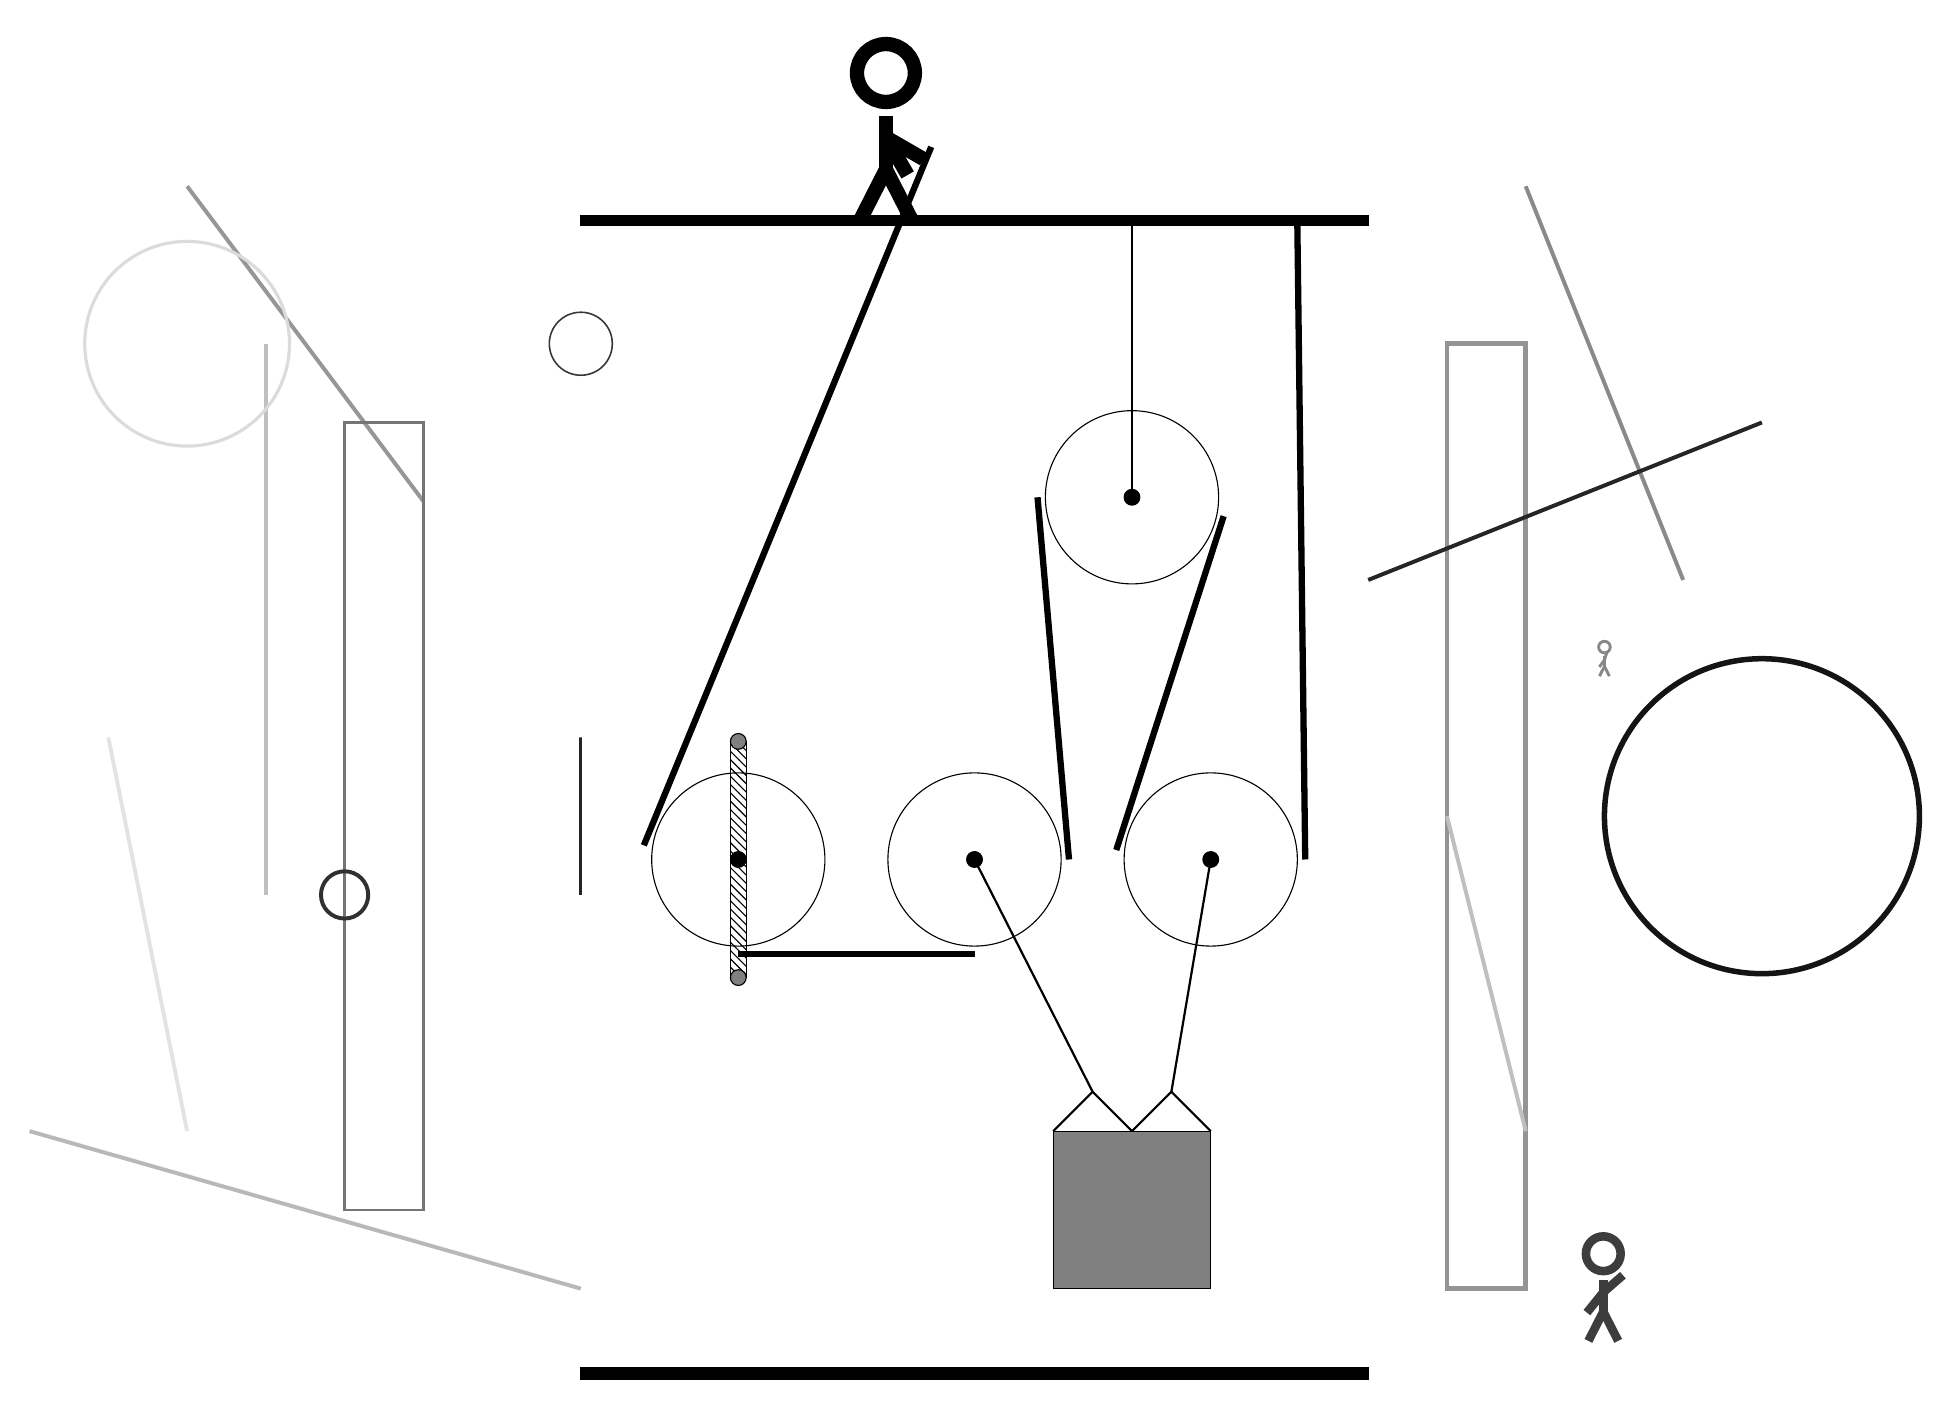
\begin{tikzpicture}
			%%%%% START %%%%%
			
			\draw[fill=black] (-4, 11.5) rectangle (6, 11.625);
			
			\draw[line width=0.6mm, color=black!42] (7, -2) rectangle (8, 10);
			
			\draw[line width=0.5mm, color=black!46](10, 7) -- (8, 12);
			\draw[line width=0.5mm, color=black!41](-6, 8) -- (-9, 12);
			\draw[line width=0.4mm, color=black!86] (-4, 3) rectangle (-4, 5);
			\draw[line width=0.5mm, color=black!11](-9, 0) -- (-10, 5);
			\draw[line width=0.5mm, color=black!28](-4, -2) -- (-11, 0);
			\draw[line width=0.5mm, color=black!85](11, 9) -- (6, 7);
			\draw[line width=0.5mm, color=black!25](-8, 10) -- (-8, 3);
			\draw [line width=0.7mm, color=black!92](11, 4) circle (2.0);
			\node[line width=0.4mm, color=black!76] at (9, -2) {\Strichmaxerl[6][51][41]};
			\draw [line width=0.4mm, color=black!14](-9, 10) circle (1.3);
			\draw[line width=0.3mm, color=black!54] (-6, -1) rectangle (-7, 9);
			\draw [line width=0.2mm, color=black!79](-4, 10) circle (0.4);
			
			\draw[line width=0.5mm, color=black!25](7, 4) -- (8, 0);
			\draw [line width=0.5mm, color=black!81](-7, 3) circle (0.3);
			\node[line width=0.5mm, color=black!47] at (9, 6) {\Strichmaxerl[2][54][72]};
			\draw [line width=0.3mm, color=black!13](-11, 1) circle (0.0);
			\draw[line width=0.5mm, color=black!97](-7, 0) -- (-7, 0);
			
			\draw (1, 3.45) circle (1.1);
			\draw[fill=black] (1, 3.45) circle (0.1);
			
			\draw (3, 8.05) circle (1.1);
			\draw[fill=black] (3, 8.05) circle (0.1);
			\draw[thick] (3, 8.05) -- (3, 11.5);
			
			\draw (4, 3.45) circle (1.1);
			\draw[fill=black] (4, 3.45) circle (0.1);
			
			\draw[thick] (4, 3.45) -- (3.5, 0.5);
			\draw[thick] (1, 3.45) -- (2.5, 0.5);
			\draw[thick]  (2, 0) -- (2.5, 0.5) -- (3, 0);
			\draw[thick]  (3, 0) -- (3.5, 0.5) -- (4, 0);
			\draw[fill=black!50] (2, 0) rectangle (4, -2);
			
			\draw (-2, 3.45) circle (1.1);
			\draw[fill=black] (-2, 3.45) circle (0.1);
			\draw[pattern=north west lines, pattern color=black] (-2.1, 4.95) rectangle (-1.9, 1.95);
			\draw[fill=black!50] (-2, 4.95) circle (0.1);
			\draw[fill=black!50] (-2, 1.95) circle (0.1);
			
			\draw[line width=0.8mm] (0.45, 12.5) -- (-3.2, 3.63);
			\centerarc[line width=0.8mm](-2, 3.45)(160:270:1.2000000000000002);
			\draw[line width=0.8mm](-2, 2.25) -- (1, 2.25);
			\centerarc[line width=0.8mm](1, 3.45)(270:360:1.2000000000000002);
			\draw[line width=0.8mm] (2.2, 3.45) -- (1.8, 8.05);
			\centerarc[line width=0.8mm](3, 8.05)(-20:180:1.2000000000000002);
			\draw[line width=0.8mm](4.164, 7.81) -- (2.8, 3.57);
			\centerarc[line width=0.8mm](4, 3.45)(160:360:1.2000000000000002);
			\draw[line width=0.8mm](5.2, 3.45) -- (5.1, 11.5);
			
			\node at (-0.07, 12.7) {\Strichmaxerl[10][120][-30]};
			
			\draw[fill=black] (-4, -3) rectangle (6, -3.15);
			
			%%%%% END %%%%%
		\end{tikzpicture}
	\end{figure}	
\end{document}